%%%%%%%%%%%%%%%%%%%%%%%%%%%%%%%%%%%%%%%%%%%%%%%%%%%%%%%%%%%%%%
%% Carlos Segarra's Beamer Presentation Template. All credits
%% to Vincent Labatut from whom I took the template and added
%% my own flavour to it. Kudos to <vincent.labatut@univ-avignon.fr>
%%%%%%%%%%%%%%%%%%%%%%%%%%%%%%%%%%%%%%%%%%%%%%%%%%%%%%%%%%%%%%
% setup Beamer
\documentclass[9pt,    % default is 11pt, use 10pt for more compact slides
%    handout,            % collapse all overlays (=animations) and video-invert console text
    english,            % presentation language (theme supports only french & english)
    xcolor=table,       % colors in the tables
    envcountsect,        % include section number in theorem numbers
    aspectratio=169     % Using 16:9 aspect ratio because 2019
]{beamer}

%%%%%%%%%%%%%%%%%%%%%%%%%%%%%%%%%%%%%%%%%%%%%%%%%%%%%%%%%%%%%%
% setup the theme
%\usepackage{au/sty/beamerthemeAU}         % no option at all
\usepackage[light]{csg-temp/sty/beamerthemeAU}   % the "light" option only changes the title and section pages

%%%%%%%%%%%%%%%%%%%%%%%%%%%%%%%%%%%%%%%%%%%%%%%%%%%%%%%%%%%%%%
% setup side notes
\usepackage{pgfpages}                                   % comment all 3 below lines to hide notes
%\setbeameroption{show notes}                           % alternate content and note slides
%\setbeameroption{show only notes}                      % only note slides
%\setbeameroption{show notes on second screen=right}    % dualscreen: right, left, top, bottom
%\usepackage{enumitem}

%%%%%%%%%%%%%%%%%%%%%%%%%%%%%%%%%%%%%%%%%%%%%%%%%%%%%%%%%%%%%%
% name of the biblatex file
\addbibresource{biblio.bib}

%%%%%%%%%%%%%%%%%%%%%%%%%%%%%%%%%%%%%%%%%%%%%%%%%%%%%%%%%%%%%%
% External Packages
\usepackage{datenumber}
\usepackage{varwidth}
\usepackage[normalem]{ulem}

% Math Mode
%\usepackage{algorithm}
%\usepackage{algorithmic}
%\usepackage{algorithm2e}
%\usepackage{multicol}
%\usepackage[noend]{algpseudocode}

%%%%%%%%%%%%%%%%%%%%%%%%%%%%%%%%%%%%%%%%%%%%%%%%%%%%%%%%%%%%%%
% title and subtitle of the presentation (the latter is optional)
\newcommand{\mainTitle}{Checkpoint/Restore of Established TCP Connections}
\newcommand{\secondTitle}{Design, Implementation, and Evaluation on runC Containers}
\subtitle{Decentralized Systems} % leave empty if no subtitle
\title[Live Migration of Containers] % leave empty for no title in footer
    {\normalsize Master in Advanced Mathematics and Mathematical Engineering \\[5pt] \Large Transparent Live Migration of Container \\ \Large Deployments in Userspace}
\subtitle{Master's Thesis - Oral Deffense} % leave empty if no subtitle
%\subtitle{Master in Research in Informatics - MIRI}
%%%%%%%%%%%%%%%%%%%%%%%%%%%%%%%%%%%%%%%%%%%%%%%%%%%%%%%%%%%%%%
% date of the presentation (leave empty for no date, default is today)
\date[July 7, 2020] % leave empty for no date in footer
    {Barcelona, Tuesday July 7, 2020}
    %{\datedayname, \today}
%%%%%%%%%%%%%%%%%%%%%%%%%%%%%%%%%%%%%%%%%%%%%%%%%%%%%%%%%%%%%%
% authors and their affiliations (the latter is optional)
\author[] % leave empty for no author in footer
{Carlos Segarra - \texttt{carlos.segarra@estudiant.upc.edu} \\ \textit{Advisor:} Jordi Guitart - \texttt{jguitart@ac.upc.edu}}
%{\inst{1} Computer Science Lab, Avignon University -- LIA EA 4128 \texttt{\{firstname.lastname\}@univ-avignon.fr}
%\and \inst{2} Institute of Disruptive Innovation, University of Excellence \texttt{\{firstname.lastname\}@univ-excell.fr}
%}
%%%%%%%%%%%%%%%%%%%%%%%%%%%%%%%%%%%%%%%%%%%%%%%%%%%%%%%%%%%%%%
% optional: additional logo (ex. lab)
%\titlegraphic{
\includegraphics[width=3cm,]{images/logo_FME.png}}
% if you want several logos, put them in a box
%\titlegraphic{\parbox{3cm}{\includegraphics[width=3cm,]{images/ceri_logo.pdf}\newline\includegraphics[width=3cm,]{images/lia_logo.pdf}}}
%%%%%%%%%%%%%%%%%%%%%%%%%%%%%%%%%%%%%%%%%%%%%%%%%%%%%%%%%%%%%%

%%%%%%%%%%%%%%%%%%%%%%%%%%%%%%%%%%%%%%%%%%%%%%%%%%%%%%%%%%%%%
% Presentation speciphic packages
% \usepackage{multicol}
% \usepackage[titles]{tocloft}
% \renewcommand{\cftchapfont}{\normalfont\bfseries}
\usetikzlibrary{decorations.pathmorphing, patterns}
\usepackage{tabularx}
\newcolumntype{L}[1]{>{\raggedright\arraybackslash}p{#1}}
\newcolumntype{C}[1]{>{\centering\arraybackslash}p{#1}}
\newcolumntype{R}[1]{>{\raggedleft\arraybackslash}p{#1}}
%%%%%%%%%%%%%%%%%%%%%%%%%%%%%%%%%%%%%%%%%%%%%%%%%%%%%%%%%%%%%

\usepackage{multimedia}
%%%%%%%%%%%%%%%%%%%%%%%%%%%%%%%%%%%%%%%%%%%%%%%%%%%%%%%%%%%%%%
\begin{document}
%%% title page
%% Outline of the presentation
% 1. Introduction - 1 slide  (include contribution list!)
% 2. Background Concepts
%   2.1. Containers - 1 slide
%   2.2. Checkpointing - 1 slide
%   2.3. CRIU - 1 slide
% 3. Implementation
%   3.0. Maybe introduce an introductory slide (?!)
%   3.1. Design Choices
%     3.1.1. Diskless Migration - 1 slide
%     3.1.2. Iterative Migration - 1 slide
%     3.1.3. TCP Connections - 1 slide
%   3.2. Implementation Details - 2 slides
% 4. Evaluation
%   4.1. Application Downtime - 1 slide
%   4.2. Scalability regarding memory size - 1 slide
% 5. Conclusions & Future Work - 1 slide

\begin{frame}
  \titlepage
\end{frame}

\begin{frame}
    \frametitle{Introduction}
    \framesubtitle{Framing the Work}

    \textbf{\textcolor{blue}{Problem Motivation:}}
    \begin{itemize}
        \item \textbf{\textcolor{blue}{Containers}} have become the go-to alternative for sandboxing and deploying distributed applications, they build on the concept of \textbf{\textcolor{blue}{namespaces}}.
        \item \href{https://en.wikipedia.org/wiki/Application_checkpointing}{Checkpointing} provides systems with \textbf{\textcolor{blue}{fault-tolerance}} and \textbf{\textcolor{blue}{state consistency}} enabling rollback and restore from previous stable versions.
        \item \textbf{\textcolor{blue}{Checkpoint-Restore in Userspace (CRIU)}} is a tool to perform checkpoint-restore of processes, transparently to the user.
        \item \textbf{\textcolor{blue}{Live migration}} consists in transparently relocating running services for improved resource-management and increased QoS.
    \end{itemize}

    \begin{columns}
        \begin{column}{.1\textwidth}
        \end{column}\hspace{-5cm}
        \begin{column}{.7\textwidth}
            \begin{alertblock}{Main Goal}
                Design, implement, and evaluate a tool for efficient live migration of running containers using \textbf{CRIU} and \textbf{runC}.
            \end{alertblock}\hfill
        \end{column}
    \end{columns}

\end{frame}

\begin{frame}
    \frametitle{Background Concepts}
    \framesubtitle{Containers and runC}

    \only<1>{
        \vspace{-15pt}

        \textcolor{blue}{\textbf{Linux Containers:}}
        \begin{alertblock}{Definition}
            A linux container is a set of processes isolated from the rest of the system.
        \end{alertblock}
        \begin{itemize}
            \item They rely on \textbf{\textcolor{blue}{namespaces}} and \textbf{\textcolor{blue}{control groups}} for fine-grained resource control.
            \item A \textbf{\textcolor{blue}{container engine}} transforms a \emph{container image} into a running process relying on a chosen \emph{runtime}.
            \item Some well-known container engines are \textsc{Docker}, \textsc{Podman}, and \textsc{Cri-O}.
        \end{itemize}
    }

    \only<1-2>{
        \textbf{\textcolor{blue}{Introduction to runC:}}
        \begin{itemize}
            \item \textbf{\textcolor{blue}{runc}} is the Open Container Initiative's (OCI) reference runtime implementation.
            \item Rather than \textbf{\textcolor{blue}{images}}, it relies on OCI bundles: \texttt{config.json} + \texttt{rootfs}.
            \item It sits at the core of most container engines as depicted in Figure 1.
        \end{itemize}
    }

    \only<2>{
        \begin{figure}[h!]
            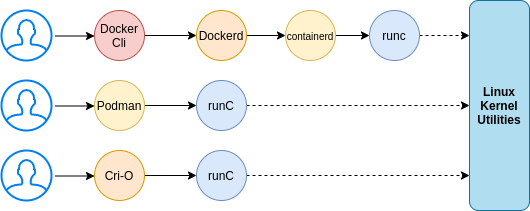
\includegraphics[width=.5\textwidth]{./images/runc.png}
            \caption{Placing runC in the call stack of different container engines.\label{fig:runc}}
        \end{figure}
    }

\end{frame}

\begin{frame}
    \frametitle{Background Concepts}
    \framesubtitle{Checkpoint-Restore and Live Migration}

    \textcolor{blue}{\textbf{Checkpoint-Restore:}}
    \begin{alertblock}{Definition (Encyclopedia of Parallel Computing)}
        Checkpointing refers to the ability to store the state of a computation in a way that allows it be continued at a later time without changing the computation's behavior.
    \end{alertblock}

    \vspace{-10pt}
    \begin{columns}[t]
        \begin{column}{.65\textwidth}
            \begin{itemize}
                \item The \textbf{\textcolor{blue}{state}} is made up of: memory, pipes, sockets, ...
                \item This state is used to \textbf{\textcolor{blue}{restore}} the process.
                \item Originated in HPC and popularized through Virtual Machines.
                \item \textbf{\textcolor{blue}{Live migration}} consists in checkpointing in an environment, and restoring in a different one.
            \end{itemize}
        \end{column}\hfill
        \begin{column}{.35\textwidth}
            \begin{figure}
                \centering
                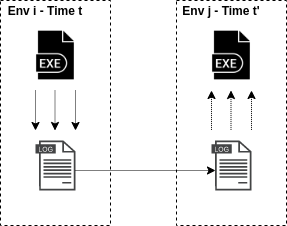
\includegraphics[width=.7\textwidth]{./images/cr.png}
                \caption{Basic working principle of live migration.}
            \end{figure}
        \end{column}
    \end{columns}

\end{frame}

\begin{frame}
    \frametitle{Background Concepts}
    \framesubtitle{\textsc{CRIU}: Checkpoint-Restore in Userspace}

    \begin{columns}[t]
        \begin{column}{.5\textwidth}
            \textbf{\textcolor{blue}{CRIU:}} Checkpoint-Restore in Userspace 
            \begin{itemize}
                \item We rely on \textbf{\textcolor{blue}{CRIU}} to perform C/R from userspace, \textbf{\textcolor{blue}{transparently}} to the user.
                \item It is an open-source, community-driven project.
                \item To \textbf{\textcolor{blue}{checkpoint}}, CRIU gathers information from different resources and dumps the content to files.
                \item To \textbf{\textcolor{blue}{restore}}, it morphs itself into the to-be restored process.
            \end{itemize}
        \end{column}
        \begin{column}{.50\textwidth}
            %\vspace{-18pt}
            \begin{table}
                \centering
                \rowcolors{1}{blue!10}{}
                {\scriptsize
                \begin{tabular}{p{1.7cm}p{1.1cm}p{1.1cm}p{1.1cm}}
                    \rowcolor{blue!50} \hline & \textbf{CRIU} & \textbf{DMTCP} & \textbf{BLCR} \\[3pt]
                    \hline \hline \textbf{Target App.} & Containers & HPC & HPC \\[3pt]
                    \textbf{Standard Kernel} & $>$ \texttt{3.11} & Yes & Yes \\[3pt]
                    \textbf{Transparency} &  Full & Pre-Load & Pre-Load \\[3pt]
                    \textbf{Unmodified App.} & Yes & Yes & No \\[3pt]
                    \textbf{Containers} & Yes & No & No \\[3pt]
                    \textbf{Distributed App.} & No & Yes & Yes \\[3pt]
                    \textbf{Open Files} & Yes & No & No \\[3pt] \hline
                \end{tabular}
                }
                \caption{Comparison with other popular C/R tools.\label{table:filter}}.
            \end{table}
        \end{column}
    \end{columns}
\end{frame}

\begin{frame}
    \frametitle{Implementation}
    \framesubtitle{Design Choices: Diskless Migration}

    \vspace{10pt}

    \textbf{\textcolor{blue}{How to reduce the impact of file I/O to disk?}}
    \begin{itemize}
        \item Employ a \emph{diskless} migration $\rightarrow$ Use a \texttt{tmpfs} mount rather than disk.
        \item Avoid writing files twice (on dump + transfer) $\rightarrow$ Use CRIU's \texttt{page-server}. 
        \item We compare a small application (100 kB, left) and a big one (1 GB, right).
    \end{itemize}

    \vspace{-5pt}

    \begin{figure}
        \centering
        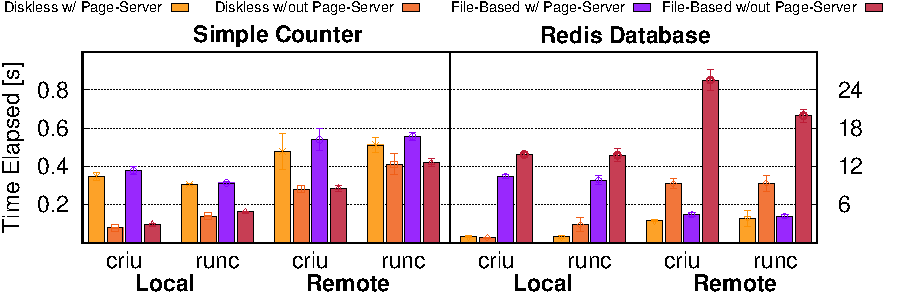
\includegraphics[width=.75\textwidth]{./figs/diskless_migration_microbenchmark.pdf}
        \caption{Diskless migration micro-benchmark.\label{fig:diskless-microbecnhmark}}
    \end{figure}
    
\end{frame}

\begin{frame}
    \frametitle{Implementation}
    \framesubtitle{Design Choices: Iterative Migration}

    \vspace{10pt}

    \textbf{\textcolor{blue}{How to minimize the application's downtime during migration?}}
    \begin{itemize}
        \item Perform iterative dumps $\rightarrow$ Use \texttt{pre-dump} and memory tracking
        \item Ensure freshness upon restore $\rightarrow$ Parent directories linked list
        \item For each application, we compare a static setting (left) and a dynamic one (right)
    \end{itemize}

    \vspace{-5pt}

    \begin{figure}
        \centering
        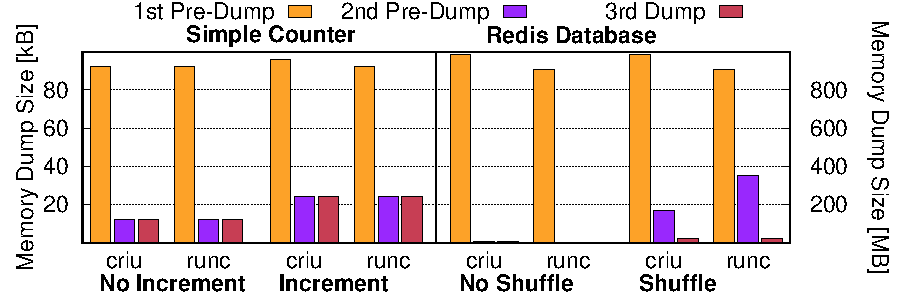
\includegraphics[width=.75\textwidth]{./figs/iterative_migration_microbenchmark.pdf}
        \caption{Iterative migration micro-benchmark.\label{fig:iterative-microbecnhmark}}
    \end{figure}
    
\end{frame}

\begin{frame}
    \frametitle{Implementation}
    \framesubtitle{Design Choices: Established TCP Connections}

    \begin{columns}
        \begin{column}{.5\textwidth}

            \vspace{-40pt}

            \textbf{\textcolor{blue}{How to migrate established TCP connections?}}
            \begin{itemize}
                \item Rely on \texttt{TCP\_REPAIR} socket option
                \item Re-create \texttt{iptables} on remote end
                \item Re-use same IP address:
                \begin{enumerate}
                    \item Using network namespaces
                    \item Using locally scoped addresses
                \end{enumerate}
                \item In the experiments we present:
                \begin{enumerate}
                    \item Downtime after an extended stop (top)
                    \item Reactivity to immediate C/R (bottom)
                \end{enumerate}
            \end{itemize}
        \end{column}
        \begin{column}{.5\textwidth}
            \begin{figure}
                \centering
                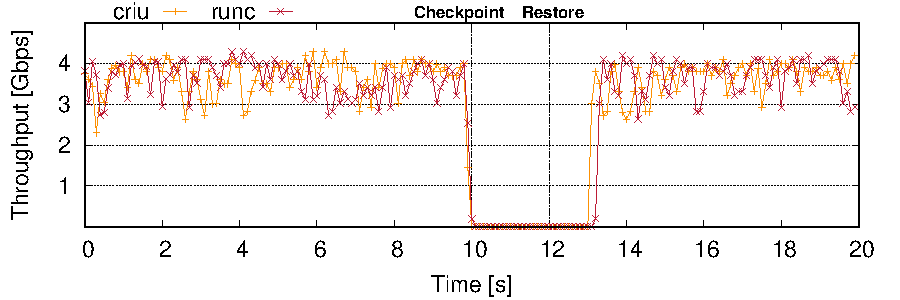
\includegraphics[width=\textwidth]{./figs/tcp_established_downtime_microbenchmark.pdf}
                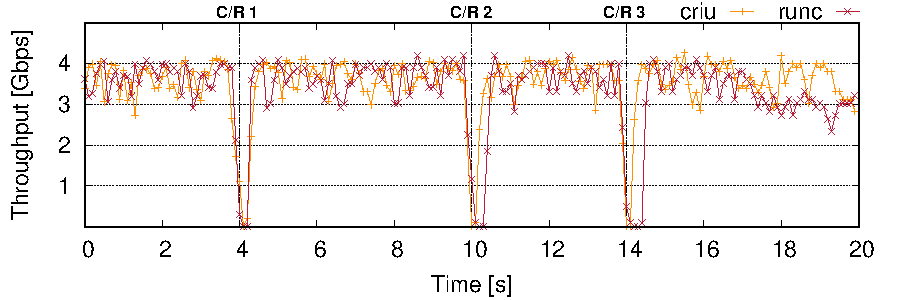
\includegraphics[width=\textwidth]{./figs/tcp_established_resolution_microbenchmark.pdf}
                \caption{TCP connections micro-benchmark.\label{fig:tcp-microbecnhmark}}
            \end{figure}
        \end{column}
    \end{columns}
    
\end{frame}

\begin{frame}
    \frametitle{Implementation}
    \framesubtitle{Putting it all together}

    \begin{columns}
        \begin{column}{.5\textwidth}

            \vspace{-40pt}

            \textbf{\textcolor{blue}{Efficient live migration of running containers:}}
            \begin{itemize}
                \item We employ a single process (no listening end on destination)
                \item We require \texttt{CAP\_SYS\_ADMIN} capabilities
                \item We make two important assumptions:
                \begin{enumerate}
                    \item The OCI bundle is available on destination
                    \item The user has SSH access to both machines 
                \end{enumerate}
                \item To run with default parameters we require:
                \begin{enumerate}
                    \item A running \texttt{runC} container's name
                    \item An IP address where to migrate it
                \end{enumerate}
            \end{itemize}
        \end{column}
        \begin{column}{.5\textwidth}
            \begin{algorithm2e}[H]
                \SetAlgoLined
                \While{size\_to\_xfer > MEMORY\_THRESHOLD}{
                    prepare\_migration()\;
                    start\_page\_server()\;
                    pre\_dump()\; 
                    transfer\_intermediate\_files()\;
                    link\_directories()\;
                }
                start\_page\_server()\;
                dump()\;
                transfer\_files()\;
                restore\_on\_remote()\;
                \caption{Main migration loop.}
            \end{algorithm2e}
        \end{column}
    \end{columns}
    
\end{frame}

\begin{frame}
    \frametitle{Evaluation}
    \framesubtitle{Application Downtime}

    \vspace{10pt}

    \textbf{\textcolor{blue}{Impact of the threshold value in total downtime:}}
    \begin{itemize}
        \item Downtime (time container is unresponsive) is the key metric of success in live migration.
        \item The \texttt{MEMORY\_THRESHOLD} becomes then a decisive design parameter.
        \item We present a macro-benchmark, studying it's impact on downtime.
    \end{itemize}

    \vspace{-5pt}

    \begin{figure}
        \centering
        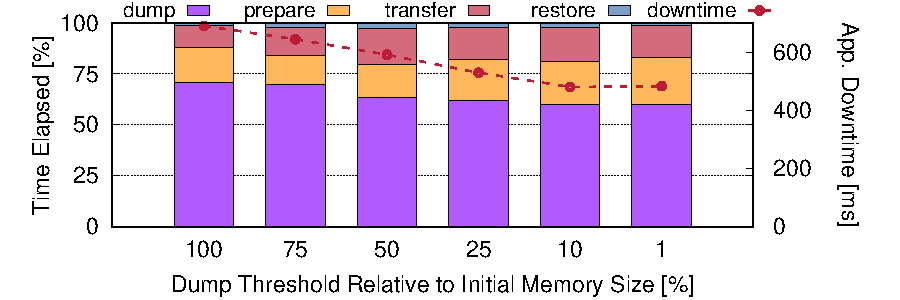
\includegraphics[width=.75\textwidth]{./figs/downtime.pdf}
        \caption{Application downtime macro-benchmark.\label{fig:diskless-microbecnhmark}}
    \end{figure}
    
\end{frame}

\begin{frame}
    \frametitle{Evaluation}
    \framesubtitle{Comparison w/ Other Techniques}

    \begin{columns}
        \begin{column}{.5\textwidth}

            \vspace{-40pt}

            \textbf{\textcolor{blue}{Comparison with other migration techniques:}}
            \begin{itemize}
                \item We compare our performance with two different settings:
                \begin{enumerate}
                    \item Naive migration: dump-transfer-restore
                    \item VM live migration: using VirtualBox's teleport
                \end{enumerate}
                \item We measure:
                \begin{enumerate}
                    \item Scalability regarding the container's memory size
                    \item Overall time elapsed (and breakdown)
                \end{enumerate}
                \item We conclude:
                \begin{enumerate}
                    \item Higher baseline than naive due to increased set-up.
                    \item $\times 1.5$ slowdown \textit{vs.} $\times 2$ for VM and $\times 10$ for naive.
                \end{enumerate}
            \end{itemize}
        \end{column}
        \begin{column}{.5\textwidth}
            \begin{figure}
                \centering
                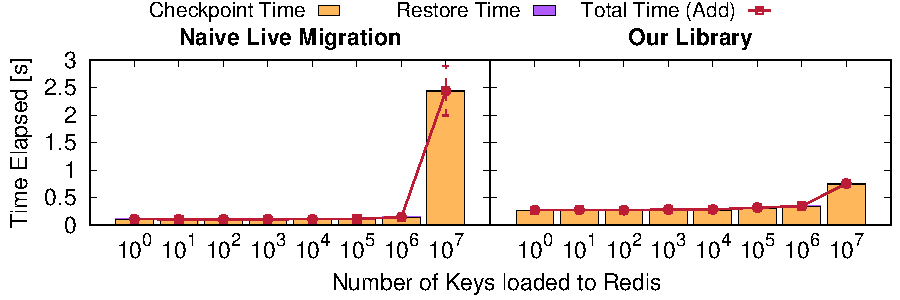
\includegraphics[width=\textwidth]{./figs/key_scalability.pdf}
                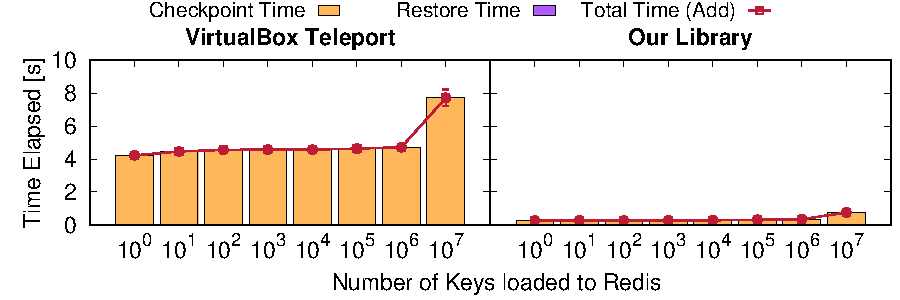
\includegraphics[width=\textwidth]{./figs/vm_teleport.pdf}
                \caption{Comparison w/ naive migration and VM migration.\label{fig:tcp-microbecnhmark}}
            \end{figure}
        \end{column}
    \end{columns}
    
\end{frame}

\begin{frame}
    \frametitle{Conclusions \& Future Work}

    \textbf{\textcolor{blue}{Conclusions}}
    \begin{itemize}
        \item[\textcolor{blue}{\textbf{+}}] Implemented an easy-to-use efficient solution.
        \item[\textcolor{blue}{\textbf{+}}] Has minimal dependencies and requires minimal set-up.
        \item[\textcolor{blue}{\textbf{-}}] Limited comparison against other solutions (several dependencies and hard to set-up).
        \item[\textcolor{blue}{\textbf{-}}] Implementation does not support all features initially planned.
    \end{itemize}

    \vspace{10pt}

    \textbf{\textcolor{blue}{To-Do List}}
    \begin{itemize}
        \item Technical Details: upon completion we plan on submitting to a specialized conference.
        \begin{enumerate}
            \item Evaluate against other live migration solutions for containers (\textit{e.g.} \texttt{P.Haul})
            \item Evaluation against other VM migration tools (\textit{e.g.} \texttt{KVM}'s or \texttt{LXC}'s)
            \item Circumvent the pre-existance requirement for OCI bundles $\rightarrow$ Generate during \texttt{pre-dump} phase.
        \end{enumerate}
        \item Future lines of work:
        \begin{enumerate}
            \item Initial goal was to support migration of distributed deployments.
            \begin{enumerate}
                \item Implement distributed checkpointing algorithms.
                \item Integrate with container orchestrators.
            \end{enumerate}
        \end{enumerate}
    \end{itemize}

\end{frame}

\begin{frame}
    \frametitle{Questions \& Discussion}

    \vspace{15pt}

    \begin{center}
        Thank you for your attention,\\[5pt]

        \Large
        \textbf{\textcolor{blue}{Observations, Doubts \& Suggestions Welcome}}\\[25pt]

        \normalsize
        Follow the development:\\ \url{https://github.com/live-containers/live-migration}\\[15pt]
        \url{carlos.segarra@estudiant.upc.edu}
    \end{center}
\end{frame}

\end{document}
